
\section{Results}
\label{sec:results}

\subsection{Main Results}

Table~\ref{tab:main_results} summarizes TSR and CAR across conditions (50 rollouts $\times$ 10 tasks per seed). $\Delta$CAR is computed against the matched-codebase Vanilla baseline (v2: $0.745 \pm 0.024$, 3 seeds, for factorial conditions above the midrule; v1: 0.780 for supplementary conditions below). Random OCC ($^\star$) uses v1 code but is included above the midrule as a factorial control; its $\Delta$CAR is omitted due to the cross-codebase baseline mismatch. Statistical comparisons use permutation tests and Hedges' $g$ (bias-corrected effect size for small samples) against the Vanilla baseline.

\textbf{Detach+LN reliably outperforms Vanilla.} The best factorial configuration, detached gradients with LayerNorm, achieves CAR $0.802 \pm 0.024$ ($n{=}3$), a $+5.7$\,pp advantage over Vanilla ($0.745 \pm 0.024$, $n{=}3$; Hedges' $g{=}1.89$, very large; bootstrap 95\% CI for $\Delta$: $[0.025, 0.089]$; Welch $t$ $p{=}0.045$).

\textbf{Two additive main effects explain the advantage.} The $2{\times}2$ factorial (Table~\ref{tab:factorial}, Figure~\ref{fig:car_factorial}b) reveals two large main effects with negligible interaction (permutation ANOVA, 10{,}000 permutations: gradient flow $p_\text{perm}{=}0.090$; normalization $p_\text{perm}{=}0.041$; interaction $p_\text{perm}{=}0.794$; Appendix~\ref{app:permutation}, Table~\ref{tab:permanova}). Bayesian model comparison provides moderate evidence favoring the additive model ($\text{BF}_{01}{=}3.5$; Appendix~\ref{app:permutation}). Parametric ANOVA yields consistent trends (Appendix~\ref{app:stat_power}). Under BatchNorm, gradient flow is associated with lower safety: Full OCC (CAR $0.725$, $\Delta{=}-2.0$\,pp) is the sole cell below Vanilla, while Detach OCC recovers ($0.767$, $\Delta{=}+2.2$\,pp); the within-row deficit is 4.2\,pp (Hedges' $g{=}0.78$, large). Under LayerNorm, gradient flow is benign: Full OCC+LN ($0.773$, $\Delta{=}+2.8$\,pp, $g{=}+0.90$) exceeds Vanilla, and Detach+LN yields the highest mean ($0.802 \pm 0.024$, $\Delta{=}+5.7$\,pp, $g{=}+1.89$). LN provides a consistent 3.5--4.8\,pp advantage over BN ($g{=}0.88$--$1.24$). The normalization main effect reaches significance under permutation testing ($p_\text{perm}{=}0.041$).

\textbf{Effect sizes and instability.} After Bonferroni correction for all pairwise comparisons, no individual Welch $t$-test reaches $\alpha{=}0.05$, consistent with $n{=}3$--$4$; we report effect sizes and planned-comparison bootstrap CIs (Appendix~\ref{app:stat_power}). The BN + gradient flow cell exhibits the highest instability ($\sigma{=}0.064$, ${\geq}\,2{\times}$ all others; $\sigma \leq 0.027$ for all other cells).

\textbf{Per-task concentration and content irrelevance.} The normalization advantage amplifies approximately fourfold on the three physically constrained tasks ($+6.9$\,pp vs.\ $+1.7$\,pp on easy tasks; T3, T5, T6; Appendix~\ref{app:per_task_factorial}), where safety margins are thinnest. Spatial content does not detectably affect outcomes: Full OCC, Random OCC, and Depth fall within cross-seed variance ($p > 0.4$, observed under v1 for Random OCC and Depth).

\textbf{BN + gradient flow is associated with training instability.} Full OCC (BN) seeds span $12.2$\,pp ($0.654$--$0.776$), more than double any other cell's range, indicating a volatile optimization landscape specific to BN + gradient flow ($\sigma \leq 0.027$ for all others vs.\ $\sigma{=}0.064$). TSR remains stable ($0.854$--$0.914$); the safety deficit does not reduce task completion.


\begin{table}[t]
\centering
\caption{Results on SafeLIBERO Level~I (10 tasks, 50 rollouts/seed). Mean $\pm$ SD across seeds. $\Delta$CAR vs.\ v2 Vanilla ($0.745$) for factorial conditions; vs.\ v1 Vanilla ($0.780$) for supplementary. $^{a}$Highest variance. $^\ddagger$2 seeds. $^\star$v1 code.}
\label{tab:main_results}
\small
\setlength{\tabcolsep}{3pt}
\begin{tabular}{llcccl}
\toprule
Flow & Norm & $n$ & CAR & TSR & $\Delta$CAR \\
\midrule
\multicolumn{6}{l}{\textit{$2{\times}2$ factorial (v2 code)}} \\
ON  & BN & 3 & $0.725 \pm 0.064^{a}$ & $0.854 \pm 0.052$ & $-$2.0 \\
OFF & BN & 4 & $0.767 \pm 0.024$ & $0.908 \pm 0.026$ & $+$2.2 \\
ON  & LN & 4 & $0.773 \pm 0.027$ & $0.914 \pm 0.049$ & $+$2.8 \\
OFF & LN & 3 & $0.802 \pm 0.024$ & $0.911 \pm 0.018$ & $+$5.7 \\
\addlinespace
---  & Vanilla & 3 & $0.745 \pm 0.024$ & $0.878 \pm 0.032$ & --- \\
\midrule
\multicolumn{6}{l}{\textit{Controls \& supplementary (v1 code)}} \\
ON  & BN (Random)$^\star$ & 3 & $0.789 \pm 0.031$ & $0.869 \pm 0.029$ & --- \\
ON  & --- (Depth)$^\star$ & 4 & $0.780 \pm 0.039$ & $0.889 \pm 0.042$ & $0.0$ \\
ON  & BN (Cutoff@15K)$^\ddagger$ & 2 & $0.782 \pm 0.031$ & $0.883 \pm 0.041$ & $+$0.2 \\
ON  & BN (Cutoff@25K)$^\ddagger$ & 2 & $0.724 \pm 0.051$ & $0.887 \pm 0.061$ & $-$5.6 \\
ON  & BN (Cutoff@35K)       & 3 & $0.779 \pm 0.017$ & $0.933 \pm 0.032$ & $-$0.1 \\
ON  & BN (Cutoff@45K)       & 1 & $0.764$           & $0.896$           & $-$1.6 \\
ON  & BN (Rev.\ Cutoff)$^\ddagger$ & 2 & $0.718 \pm 0.025$ & $0.839 \pm 0.072$ & $-$6.2 \\
\bottomrule
\end{tabular}
\end{table}

\begin{table}[t]
\centering
\caption{$2{\times}2$ factorial: normalization type $\times$ gradient flow (all v2 data). Two main effects: gradient flow under BN $g{=}0.78$ (large); normalization effect $g{=}0.88$--$1.24$ (large to very large). BN + gradient flow is the sole cell below Vanilla. Interaction $p_\text{perm}{=}0.794$. $\text{BF}_{01}{=}3.50$ (moderate evidence for additivity).}
\label{tab:factorial}
\begin{tabular}{lccc}
\toprule
 & Gradient ON & Gradient OFF & $\Delta$(ON$-$OFF) \\
\midrule
BatchNorm    & Full OCC (0.725) & Detach OCC (0.767) & $-$4.2 \\
LayerNorm    & Full OCC+LN (0.773) & Detach+LN (0.802) & $-$2.9 \\
\midrule
$\Delta$(BN$-$LN) & $-$4.8 ($g{=}{-}0.88$) & $-$3.5 ($g{=}{-}1.24$) & --- \\
\bottomrule
\end{tabular}
\end{table}

% Old Fig 2 (factorial standalone) — merged into fig:factorial_gradient below
% \begin{figure}[t]
% \centering
% 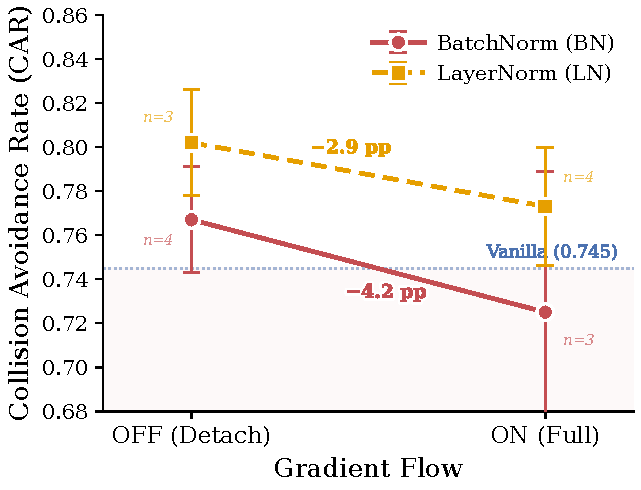
\includegraphics[width=\columnwidth]{figures/factorial_2x2_pb.pdf}
% \caption{...}
% \label{fig:factorial_old}
% \end{figure}

\begin{figure*}[t]
\centering
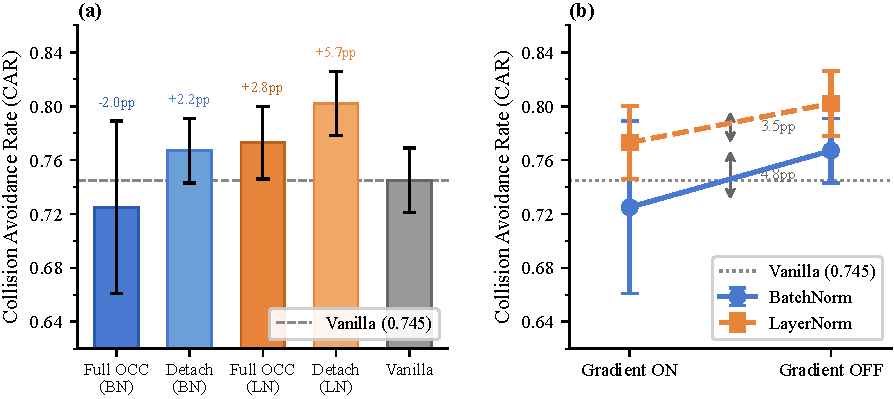
\includegraphics[width=\textwidth]{figures/fig_car_factorial_combined.pdf}
\caption{(a)~Only BN + gradient flow falls below Vanilla. Detach+LN achieves the highest CAR ($0.802{\pm}0.024$, $n{=}3$), consistently outperforming Vanilla ($0.745$; Hedges' $g{=}1.89$). Error bars: cross-seed SD. (b)~Classic interaction plot: near-parallel lines indicate negligible interaction ($p_\text{perm}{=}0.794$). LN consistently outperforms BN by 3.5--4.8\,pp regardless of gradient flow. Only BN + gradient ON falls below Vanilla.}
\label{fig:car_factorial}
\end{figure*}

\subsection{Factorial Interpretation}

\textbf{Gradient flow is associated with lower safety under BatchNorm but not under LayerNorm.} Full OCC (BN) is the sole cell below Vanilla ($\Delta{=}-2.0$\,pp), while all other cells exceed it (Table~\ref{tab:factorial}). Detach+LN yields the highest mean ($0.802$, $g{=}+1.89$; bootstrap 95\% CI for $\Delta$: $[0.025, 0.089]$). This is a practical threshold crossing rather than a statistical interaction ($\eta^2{=}0.005$).

\textbf{Temporal dynamics.} Cutoff conditions illuminate when gradient flow's association with lower safety emerges. Cutoff@15K ($\Delta{=}+0.2$\,pp) performs near Vanilla, while Cutoff@25K exhibits a deficit ($\Delta{=}-5.6$\,pp, $n{=}2$) and Cutoff@35K returns to baseline ($\Delta{=}-0.1$\,pp). Cutoff@45K ($\Delta{=}-1.6$\,pp, single seed) falls between these extremes. This non-monotonic pattern suggests that the critical window for the gradient flow safety deficit is not simply cumulative exposure but depends on the training phase. Reverse Cutoff (gradient flow only after step 35K, $n{=}2$) yields the lowest supplementary CAR ($\Delta{=}-6.2$\,pp); late-stage gradient flow, when the model is refining action predictions, is associated with substantially worse outcomes than early exposure during initial representation learning. However, temporal conditions use 1--3 seeds (v1); these observations are preliminary.

\subsection{Gradient Dynamics}

Gradient analysis (Figure~\ref{fig:gradient_analysis}) examines the mechanism through which auxiliary heads affect safety. All gradient norms are computed with respect to the L1 action loss (action tokens only).

\begin{figure*}[t]
\centering
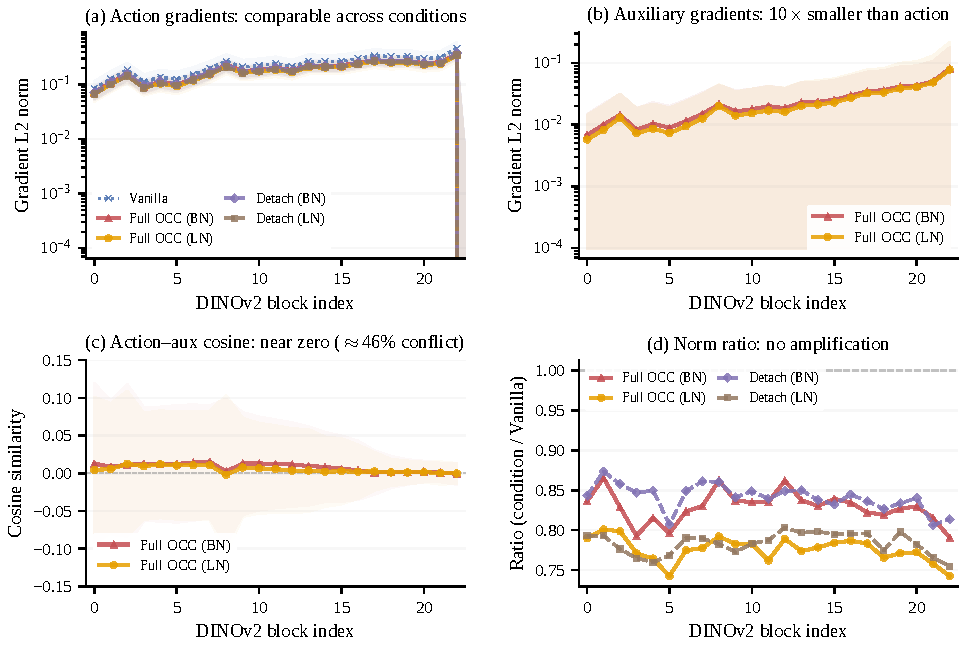
\includegraphics[width=\textwidth]{figures/gradient_analysis_v2_combined.pdf}
\caption{Gradient dynamics (v2, seed 42, 200 batches at 50K; Random OCC data obtained under v1 codebase). Action gradient norms are comparable across conditions, ruling out amplification. Action--auxiliary cosine similarity is near zero (${\approx}$46\% conflict rate), consistent with orthogonality.}
\label{fig:gradient_analysis}
\end{figure*}

\textbf{Gradient orthogonality rules out direct conflict.} Action--auxiliary gradient cosine similarity is near zero across all encoder layers for both Full OCC and Random OCC (Figure~\ref{fig:gradient_analysis}), with conflict rates of ${\approx}$46\%. Action loss gradient norms are comparable across Vanilla and gradient-flow conditions (Figure~\ref{fig:gradient_analysis}), ruling out gradient amplification. Both patterns are identical for structured and random labels, consistent with the behavioral finding that spatial content did not detectably affect outcomes. (Random OCC gradient data were obtained under the v1 codebase; the v2 gradient analysis covers all four factorial conditions and Vanilla, each using a v2-trained checkpoint.)

\textbf{Mechanism remains open.} Neither gradient conflict nor amplification explains the effect. CKA analysis~\cite{kornblith2019similarity} confirms intact encoder representations (CKA $\geq$ 0.95 across all layers), localizing the safety deficit to optimization dynamics---likely subtle LoRA adapter weight differences invisible to representational similarity measures.

Additional observations (per-task breakdown, depth comparison, and temporal dynamics) are in Appendix~\ref{app:additional}.
